% Created 2024-03-07 Thu 15:43
% Intended LaTeX compiler: pdflatex
\documentclass[11pt]{article}
\usepackage[utf8]{inputenc}
\usepackage[T1]{fontenc}
\usepackage{graphicx}
\usepackage{longtable}
\usepackage{wrapfig}
\usepackage{rotating}
\usepackage[normalem]{ulem}
\usepackage{amsmath}
\usepackage{amssymb}
\usepackage{capt-of}
\usepackage{hyperref}
\usepackage[margin=0.5in]{geometry}
\usepackage{tikz}
\date{}
\title{Does Identity Matter?}
\hypersetup{
 pdfauthor={Rudolf Jovero},
 pdftitle={Does Identity Matter?},
 pdfkeywords={},
 pdfsubject={},
 pdfcreator={Emacs 29.1 (Org mode 9.6)}, 
 pdflang={English}}
\begin{document}


\section*{Does Personal Identity Matter?}
\label{sec:org165cbdf}
Science fiction has provided us with many cases where the concept of the self is challenged.

\subsubsection*{Sci-Fi}
\label{sec:orgcc1afd2}
\begin{itemize}
\item Teleportation accidents (\emph{Star Trek}) -
\label{sec:org65c92cf}
deconstruction fails, or reconstruction occurs in multiple instances.

\item Mind duplication technology (\emph{Altered Carbon}, \emph{Black Mirror}) -
\label{sec:org7904153}
minds are saved and duplicated for purposes of replication later.
\end{itemize}

\subsubsection*{In Real Life}
\label{sec:orgb589a9f}
There have been instances where people survive with only half a brain, or where the corpus callosum was severed to treat epilepsy.
In the latter case it seemed like there were two sets of consciousnesses/mentalities.

\section*{Scope}
\label{sec:orge81f7da}
\subsection*{Self resides in the mind}
\label{sec:orgd13a34e}
For the purpose of this discussion,
we will assume the self is contained in our mental properties.
Locke would argue the self resides in our memory, Hume would say what we call the self is a bundle of impressions.

While genetic and neural dispositions can instantiate a self, in terms of changes to the self, we will assume that the self need not be continued on the same physical hardware it originated from.

\subsection*{Personal Identity over time}
\label{sec:org3ba2b1b}
Derek Parfit developed a lot of the modern discourse on Personal Identity.
He was concerned with identity over time, not identity in an instance.
Concepts such as nationality, sexuality, and sex and gender can be considered impressions/propositional attitudes. in an instant, and we'll treat them all as some of the aspects of the self that can vary over time.
We're more concerned with how the self changes over time.

\subsubsection*{Survival of the self}
\label{sec:org167bce4}
We're concerned with whether an entity called the self persists through given scenarios.
Identity \(\rho\) is a specific relation (\(\rho\)) that does not seem to apply in all cases,
yet it seems we would agree that a self persists even if an identity does not.

\subsubsection*{Identity \(\rho\)}
\label{sec:org9f25fe0}
Reflexive \[x=x\]
Symmetric \[x=y \rightarrow y=x\]
Transitive \[x=y \wedge y=z \rightarrow x=z\]
Personal Identity is a numeric identity, we're concerned about whether we can call a person the same person throughout time.
A belief in self that depends on the identity \(\rho\) implies that there is an entity that meets these criteria when a self survives, and no existence of one when a self does not survive.
These properties imply identity as an all-or-nothing, one-to-one relation.
This is the notion of the self that Parfit challenges.

\section*{Thought Experiment}
\label{sec:orgce83243}
The main thought experiment we're concerned with are cases of psychological fission.
If we have a mind that divides into multiple instances, can we really say anything about identity?


\subsection*{Psychological fission}
\label{sec:org6f4e3b1}
The case of fission targets the one-to-one aspect of Personal Identity and the self.
It also introduces the concept of Psychological Continuity.
\\\empty
\\\empty
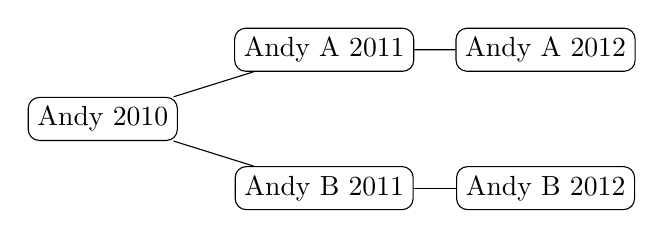
\begin{tikzpicture}
[sibling distance=5em, level distance=8em, grow=right,
every node/.style={shape=rectangle, rounded corners, draw, align=center}]
\node{Andy 2010}
  child{node{Andy B 2011}
    child{node{Andy B 2012}}}
  child{node{Andy A 2011}
    child{node{Andy A 2012}}};
\end{tikzpicture}
\subsubsection*{Interpretations:}
\label{sec:org25afbcd}
\begin{itemize}
\item Andy died in 2011 -
\label{sec:org915f9e2}
So a double success is a failure?

\item Either Andy A or Andy B is the only one identical to Andy 2010 -
\label{sec:orgb4a4466}
How do you get to decide who the identical one is?

\item Andy A and Andy B are both Andy 2010 -
\label{sec:org8d8d99a}
If one kills the other, is it both a murder and a suicide?
\item Abandon Personal Identity as a necessary relation -
\label{sec:org2e0b1d0}
\emph{Psychological Continuity} is a better relation to focus on. Personal Identity is just a special case of \emph{Psychological Continuity} where there is no branching.
\end{itemize}

\subsection*{Psychological Fusion}
\label{sec:orgf9b7212}
\\\empty
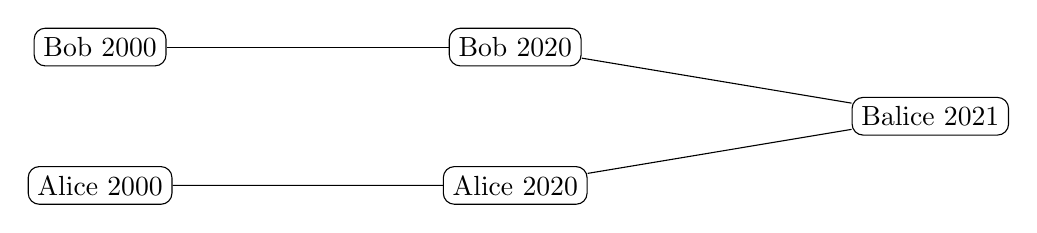
\begin{tikzpicture}
[sibling distance=5em, level distance=15em, grow=left,
every node/.style={shape=rectangle, rounded corners, draw, align=center}]
\node{Balice 2021}
  child{node{Bob 2020}
        child{node{Bob 2000}}
}
  child{node{Alice 2020}
        child{node{Alice 2000}}
    };
\end{tikzpicture}
\\\empty

In psychological fusion, the aspect of identity that is challenged is all-or-nothing.
In fission we showed that what matters does not need to be one-to-one.
Also Balice would not have all of Bob's or all of Alice's impressions/propositional attitudes.
Balice is \emph{Psychologically Connected} with memories/attitudes of both Bob and Alice.
We don't need a fusion case to talk about \emph{Psychological Connectedness}.
\\\empty
\\\empty

\begin{tikzpicture}
[sibling distance=5em, level distance=15em, grow=left,
every node/.style={shape=rectangle, rounded corners, draw, align=center}]
\node{Leela 2040}
  child{node{Leela 2030}
        child{node{Leela 2020}
            child{node{Leela 2010}
}}};
\end{tikzpicture}
\section*{Implications}
\label{sec:org4369775}
\subsubsection*{What is love?}
\label{sec:org8333811}
\subsubsection*{Who is responsible? What is remorse good for?}
\label{sec:org5be5825}
\subsubsection*{What does self interest mean without identity?}
\label{sec:orgb98366e}
Is it morally right to decide which branch of yourself gets a better life?
\end{document}